%
%  Search for Rare Higgs Decays
%

I begin with a brief discussion of the motivation behind looking for rare Higgs decays like $H \rightarrow \rho+\gamma$ and $H \rightarrow \phi+\gamma$, specifically via the associated $WH$ rather than direct production. Then, I outline the event selection methods and relevant backgrounds. Finally, I describe the Boosted Decision tree we used in detail, followed by the results of the analysis.

\begin{section}{Motivation}

The branching ratios for the $H \rightarrow \phi+\gamma$ and $H \rightarrow \rho+\gamma$ decays are expected to have a lower bound of $8.8 \times 10^{-4}$ and $4.8 \times 10^{-4}$  respectively\cite{cite-rpg-brs}. Put simply, they are \textit{very} rare - so rare, in fact, that they have never been directly observed. Furthermore, by any measure, these decays should never be detectable at current, human-reachable energies, that is, unless there are yet-undiscovered processes that enhance the rate of either of these decays. This implies that this measurement is experimentally exciting, because any significant measurement of the production of $\rho$ or $\phi$ mesons would be direct evidence of the existence of new physics. At the same time, if no $\rho$ or $\phi$ mesons are found, then the branching ratio of either decay mode can be pushed farther back, depending on the detector's sensitivity to the signature.

Now, ideally, we would search for these decays via \textit{direct} production, that is, when a Higgs boson is produced by gluon-gluon fusion (Fig. \ref{fig:direct-prod}), then decays to a photon and a $\phi$ or $\rho$ meson. However, CMS does not have a dedicated trigger for detecting pions or kaons (the final-state products of the $\phi$ and $\rho$ mesons respectively), so the only possibly detectable particle would be the photon. However, since the Higgs mass is 125 GeV, the photon and meson both have a momentum of approximately 60 GeV at most, so the photon is well below the threshold of the CMS single photon trigger\cite{cite-hlt}. Therefore, we chose an associate production mode, namely, $W^{\pm}+H$ (Fig. \ref{fig:whiggs-prod}), where $W \rightarrow \ell^{\pm}+\nu_{\ell}$. We can easily trigger on the leptons produced by the $W$ boson, and the Higgs comes for free. At the same time, we lose a \textit{lot} of signal, since this process is far more rare. We also have to deal with more background, since we are including more particles in the signature we are searching for. Ultimately these consequences consolidate into an overall loss of sensitivity, but alternative associated productions ($Z+H$, for instance) face similar challenges.

\begin{figure}[htb]
\begin{center}
% Naming convention:
%    <above/below : a/b><level: #>_<#cm from origin>
%    Examples:
%       a2_0 = above, level 2, at origin
%       b3_1 = below, level 3, 1cm from origin

\begin{tikzpicture}
  \begin{feynman}
    
    % START: Horizon ---------------------------------
    \vertex (horizon);
    \vertex[right=5cm of horizon] (hz_5);
    \vertex[right=7cm of horizon] (hz_7);
    % END: Horizon -----------------------------------
    
    % START: Above -----------------------------------
    % Level +3
    \vertex[above=3cm of horizon] (a3);
    \vertex[right=13cm of a3] (a3_13) {\(u,s\)};
    % Level +2
    \vertex[above=2cm of horizon] (a2);
    \vertex[left=1cm of a2] (1_a2) {\(g\)};
    \vertex[right=2cm of a2] (a2_2);
    \vertex[right=10cm of a2] (a2_10);
    \vertex[right=12cm of a2] (a2_12);
    % Level +1
    \vertex[above=1cm of horizon] (a1);
    \vertex[right=13cm of a1] (a1_13) {\(\overline u,\overline s\)};
    % END: Above -------------------------------------
    
    % START: Below -----------------------------------
    % Level -2
    \vertex[below=2cm of horizon] (b2);
    \vertex[left=1cm of b2] (1_b2) {\(g\)};
    \vertex[right=2cm of b2] (b2_2);
    \vertex[right=10cm of b2] (b2_10);
    \vertex[right=13cm of b2] (b2_13) {\(\gamma\)};

    \diagram* {
      {[edges=gluon]
        (1_a2) -- (a2_2),
        (1_b2) -- (b2_2),
      },
      
      (a2_2) -- [fermion, edge label=\(t\)] (hz_5),
      (b2_2) -- [anti fermion, edge label=\(\overline t\)] (hz_5),
      (a2_2) -- [anti fermion, edge label=\(\overline t\)] (b2_2),
      
      (hz_5) -- [scalar, edge label=\(H\)] (hz_7),
      
      (hz_7) -- [fermion, edge label=\(t\)] (a2_10),
      (b2_10) -- [anti fermion, edge label=\(\overline t\)] (a2_10),
      (hz_7) -- [anti fermion, edge label=\(\overline t\)] (b2_10),
      
      (a2_10) -- [photon, edge label=\(\gamma\)] (a2_12),
      (a2_12) -- [fermion] (a3_13),
      (a2_12) -- [anti fermion] (a1_13),
      
      (b2_10) -- [photon] (b2_13),
    };
    
    \draw [decoration={brace}, decorate] (a3_13.north east) -- (a1_13.south east)
          node [pos=0.5, right] {\(\rho, \phi\)};
  \end{feynman}
\end{tikzpicture}
\end{center}
\caption{Feynman diagram\cite{cite-tikz-feynman} for primary mechanism of the direct production of the Higgs boson at the LHC where $H \rightarrow \rho+\gamma$ or $H \rightarrow \phi+\gamma$.}
\label{fig:direct-prod}
\end{figure}

\begin{figure}[htb]
\begin{center}
% Naming convention:
%    <above/below : a/b><level: #>_<#cm from origin>
%    Examples:
%       a2_0 = above, level 2, at origin
%       b3_1 = below, level 3, 1cm from origin

\begin{tikzpicture}
  \begin{feynman}
    
    % START: Horizon ---------------------------------
    \vertex (horizon);
    \vertex[right=1cm of horizon] (hz_1);
    \vertex[right=3cm of horizon] (hz_3);
    \vertex[right=9cm of horizon] (hz_9) {\(u,s\)};
    % END: Horizon -----------------------------------
    
    % START: Above -----------------------------------
     % Level +3
    \vertex[above=3cm of horizon] (a3_0);
    \vertex[right=6cm of a3_0] (a3_7) {\(\ell^{\pm}\)};
    % Level +2
    \vertex[above=2cm of horizon] (a2_0);
    \vertex[right=5cm of a2_0] (a2_5);
    % Level +1
    \vertex[above=1cm of horizon] (a1_0);
    \vertex[left=1cm of a1_0] (a1_1) {\(q\)};
    \vertex[right=6cm of a1_0] (a1_7) {\(\nu_{\ell}\)};
    % END: Above -------------------------------------
    
    % START: Below -----------------------------------
    % Level -1
    \vertex[below=1cm of horizon] (b1_0);
    \vertex[left=1cm of b1_0] (b1_1) {\(\overline q\)};
    \vertex[right=7cm of b1_0] (b1_7);
    \vertex[right=8cm of b1_0] (b1_8);
    % Level -2
    \vertex[below=2cm of horizon] (b2_0);
    \vertex[right=5cm of b2_0] (b2_5);
    \vertex[right=9cm of b2_0] (b2_9) {\(\overline u,\overline s\)};
    % Level -3
    \vertex[below=3cm of horizon] (b3_0);
    \vertex[right=7cm of b3_0] (b3_7);
    \vertex[right=9cm of b3_0] (b3_9) {\(\gamma\)};

    \diagram* {
      (a1_1) -- [fermion, edge] (hz_1),
      (b1_1) -- [anti fermion, edge] (hz_1),
      
      (hz_1) -- [boson, edge label=\(W^{*}\)] (hz_3),
      (hz_3) -- [boson, edge label=\(W^{\pm}\)] (a2_5),
      (hz_3) -- [scalar, edge label=\(H\)] (b2_5),
      
      {[edges=fermion]
        (a2_5) -- (a3_7),
        (a2_5) -- (a1_7),
      },
      
      (b2_5) -- [fermion, edge label=\(t\)] (b1_7),
      (b1_7) -- [fermion, edge label=\(t\)] (b3_7),
      (b2_5) -- [anti fermion, edge label=\(\overline t\)] (b3_7),
      
      (b1_7) -- [photon, edge label=\(\gamma\)] (b1_8),
      (b3_7) -- [photon] (b3_9),
      
      (b1_8) -- [fermion, edge] (hz_9),
      (b1_8) -- [anti fermion, edge] (b2_9),
    };
    
    \draw [decoration={brace}, decorate] (hz_9.north east) -- (b2_9.south east)
          node [pos=0.5, right] {\(\rho, \phi\)};
  \end{feynman}
\end{tikzpicture}
\end{center}
\caption{Feynman diagram\cite{cite-tikz-feynman} for primary mechanism of the associated $WH$ production at the LHC studied in this analysis.}
\label{fig:whiggs-prod}
\end{figure}
\end{section}

\begin{section}{Event Selection}
\begin{subsection}{Data Aquisition}
The analysis begins with data based on a sample of proton-proton collisions collected by the Compact Muon Solenoid (CMS) detector in the LHC. ``Interesting'' events are selected by the first level of the CMS trigger system which uses information from the detector's calorimeters and muon detectors to select events for analysis in a fixed time interval of less than 4 $\mu s$. These events are then further processed by a high-level trigger processor farm, which decreases the event rate from around 100 kHz to less than 1 kHz, before the data is stored. Finally, the particle-flow algorithm reconstructs and identifies all particles from the events selected by the CMS trigger system. With the data properly processed and promptly reconstructed ``online,'' further analysis can be carried out ``offline.''
\end{subsection}
\begin{subsection}{Baseline Selection}
To start offline analysis, we first apply a baseline selection on data and Monte Carlo samples to filter out particularly irrelevant events. First, we require at one ``good" lepton, qualified as:
\begin{itemize}
    \item $p_{T}(\ell^{\pm}) > 10\textnormal{ GeV}$
    \item $\eta(\ell^{\pm}) < 2.4$
    \item $ID(e^{\pm})$ \verb|HAD_medium_noiso_v5|
    \item $ID(\mu^{\pm})$ \verb|isMediumMuonPOG|
    \item $I_{rel}(e^{\pm}) < 0.1$ using \verb|elMiniRelIsoCMS3_EA|
    \item $I_{rel}(\mu^{\pm}) < 0.2$ using \verb|muMiniRelIsoCMS3_EA|
\end{itemize}

\noindent We also require one good photon, qualified as:
\begin{itemize}
    \item $p_{T}(\gamma) > 20\textnormal{ GeV}$
    \item $\eta(\gamma) < 2.5$
    \item $ID(\gamma)$ \verb|isMediumPhotonPOG_Fall17V2|
    \item $I_{rel}(\gamma) < 0.06$
    \item $\Delta R(\gamma, e^{\pm}) < 0.2$
\end{itemize}
\noindent where if two or more good $\ell$ or $\gamma$ candidates are found, the candidate with the highest $p_{T}$ is selected. Finally, we require two, oppositely charged hadrons. This is complicated by the fact that CMS does not distinguish pions and kaons in reconstruction, but we begin by requiring one good hadron ($h$) candidate pair ($h^{+}, h^{-}$), which describe some unidentified mother meson ($M$), qualified as:
\begin{itemize}
    \item $p_{T}(h^{\pm}) > 10\textnormal{ GeV}$
    \item $\eta(h^{\pm}) < 2.4$
    \item $h^{+}, h^{-}$ from the same primary vertex
    \item $I_{rel}(M) < 0.06$
    \item $\Delta R(h^{+}, h^{-}) < 0.1$
\end{itemize}
\noindent where $I_{rel}(M) = \frac{max(I(h^{+}), I(h^{-}))}{p_{T}(M)}$. Now, as mentioned previously, the the exact identity of these hadrons is ambiguous. They are saved, by default, as pions, so their four-momenta are all constructed using the pion's mass contribution to the energy component. We add these to form the $\rho$-candidate four-momentum and designate it as the ``pion hypothesis." Then, we manually set the energy-components of the hadron four-momenta using the kaon mass, add them to form the $\phi$-candidate four-momentum, and designate it as the ``kaon hypothesis." If two or more of either hypothesis is found, we select the hypothesis that is closest to the true, respective mass. This leads to the possibility of biasing the data, but we avoid this later by rejecting any events with more than one meson candidate.
\end{subsection}
\end{section}

\begin{section}{Backgrounds}
We are looking for two final-state particles: one photon and one $\rho$ or $\phi$ meson. However, there are a number of processes besides the Higgs decays we are interested in that could present the same signature. In the following paragraphs, I describe how we might get false photons and false mesons that, when combined, present a signal-like signature.

We may get a real, prompt photon in W events where a photon was radiated by one of the initial-state quarks (Fig. \ref{fig:whiggs-prod}). We might also get a fake photon from misidentified jets in W events. Finally, from Z events, we can get fake photons from misidentified electrons.

Fake mesons may be produced by any two tracks that happen to both be isolated from all particles other than each other and have a combined invariant mass that lands in the $\rho$ or $\phi$-meson Breit-Wigner lineshapes.
\end{section}

\begin{section}{Boosted Decision Tree}
\begin{subsection}{Training}
Prior to training, we made the following cuts that prevent over-training the BDT by essentially pre-training it to cut on each respective variable:

\begin{itemize}
    \item $1.0 < m_{\phi} < 1.04\textnormal{ GeV}$
    \item $80 < m_{Z} < 95\textnormal{ GeV}$
\end{itemize}

\noindent where each was chosen because of the narrow width of their distributions. Then, because BDT's are vulnerable to low statistics, we also added several extraneous, orthogonal datasets that were unnecessary for the greater analysis, but served as useful, accurate background shapes. Ultimately, we gave BDT 40563 training and 13522 testing events.

We began with the XGBoost python package, a well-known implementation of gradient-boosted decision trees. Twenty-two features were selected, from those saved during the baseline selection step, based on their merit as variables that are reasonably uncorrelated to the signal region (reconstructed Higgs boson mass). The unweighted distributions for all input features are shown in Fig. \ref{fig:bdt-vars}, but they are also listed below divided into categories for brevity and later reference:
\begin{enumerate}[(i.)]
    \item Missing Transverse Energy ($\slashed{E}_{T}$):
    \begin{itemize}
        \item $p_{T}(\slashed{E}_{T})$
        \item $\varphi(\slashed{E}_{T})$
    \end{itemize}
    \item Basic Kinematics:
    \begin{itemize}
        \item $p_{T}(\gamma)$, $p_{T}(\phi)$
        \item $\eta(\gamma)$, $\eta(\phi)$, $\eta(\ell^{\pm})$
        \item $\varphi(\gamma)$, $\varphi(\phi)$, $\varphi(\ell^{\pm})$
        \item $\Delta R(\gamma, \ell^{\pm})$, $\Delta R(\phi, \gamma)$, $\Delta R(K^{+}, K^{-})$
    \end{itemize}
    \item Masses:
    \begin{itemize}
        \item $m_{Z}$, $m_{\phi}$
    \end{itemize}
    \item MELA ``Magic" Angles:
    \begin{itemize}
        \item $\Phi$, $\Phi_{1}$
        \item $\cos\theta_{1}$, $\cos\theta_{2}$, $\cos\theta^{*}$
    \end{itemize}
\end{enumerate}

\noindent Now, there are some important clarifications to make here. First, we scaled all $p_{T}$ quantities that are correlated to the Higgs and input into the BDT by the Higgs mass. Second, $\varphi$ refers to the azimuthal angle (see Fig. \ref{fig:cms-coords}) which is not to be confused with the $\phi$-meson. Finally, we calculated the quantities listed under (iv.) using MELA\cite{cite-mela} (all angles used are illustrated in Fig. \ref{fig:magic-angles}).

\begin{figure}[htb]
\begin{center}
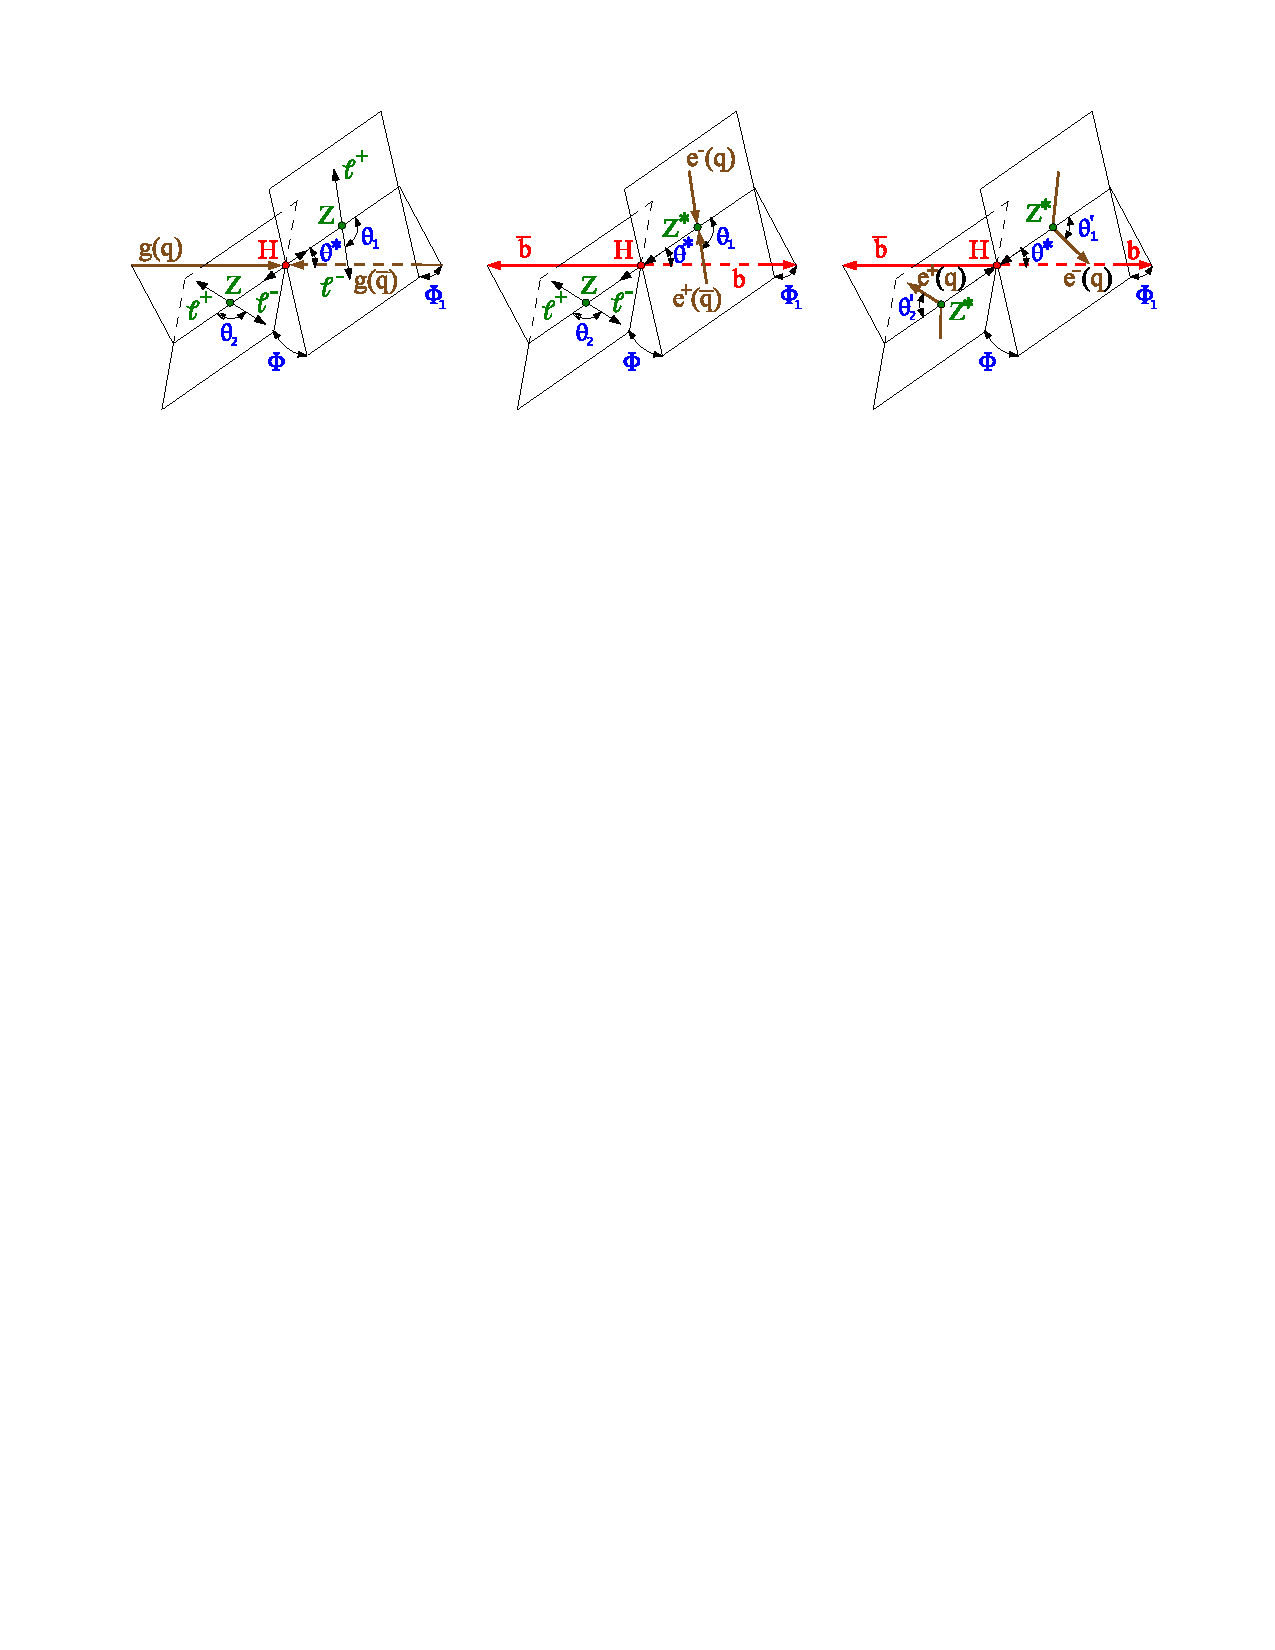
\includegraphics[width=.95\linewidth]{Dissertation/fig/magic-angles.pdf}
\end{center}
\caption{Diagram due to Anderson et. al. \cite{magic-angles-cite} of Higgs-frame angles used for BDT training. The center diagram is most relevant under the following replacements: $Z, Z^*$ to $W, W^*$, $b, \bar{b}$ to $\rho/\phi, \gamma$; $\ell^+,\ell^-$ to $e^-/\mu^-, \nu_e/ \nu_\mu$.}
\label{fig:magic-angles}
\end{figure}

With these features properly defined, we ran the BDT for 200 training rounds with the following model hyperparameters selected to maximize BDT efficiency without overtraining (See Fig. \ref{fig:bdt-knobs} for hyperameter definitions):
\begin{itemize}
    \item \verb|objective| = 'binary:logistic'
    \item \verb|eta| = 0.1
    \item \verb|max_depth| = 3
    \item \verb|verbosity| = 1
    \item \verb|nthread| = 12
    \item \verb|eval_metric| = "auc"
    \item \verb|subsample| = 0.6
    \item \verb|alpha| = 8.0
    \item \verb|gamma| = 2.0
    \item \verb|lambda| = 1.0
    \item \verb|min_child_weight| = 1.0
    \item \verb|colsample_bytree| = 1.0
\end{itemize}

\end{subsection}
\begin{subsection}{Performance and Validation}
We determined satisfactory performance by evaluating the BDT's ROC curves for testing and training (Fig. \ref{fig:bdt-performance}) as well as the sanity of the BDT's feature rankings (Fig. \ref{fig:bdt-vars}). We also checked for background sculpting by two methods. First, we looked at the plot of the BDT scores versus the reconstructed Higgs mass (Fig. \ref{fig:bdt-bkgsculpt1}). A correlation between high BDT scores and the known Higgs mass (125 GeV) would indicate that the BDT was simply learning and cutting on the reconstructed Higgs mass and thus sculpting the background. Second, we directly evaluated the background and signal distributions before and after making a tight cut ($D > 0.9$) on the BDT discriminant, where an artificial peak of the background inside of the signal region would directly show that the BDT was sculpting the background. We required that the BDT pass these two tests before proceeding to use it in the rest of the analysis.

\begin{figure}[htb]
\begin{center}
\begin{tabular}{llll}
\toprule
cut &       gain &       cover &  weight \\
\midrule
$I_{rel}(\phi)$ &  64.823995 &  410.500067 &      57 \\
$\Delta R(K^{+}, K^{-})$ &  49.762952 &  315.353542 &     143 \\
$m_{Z}$ &  34.554528 &  292.716951 &     107 \\
$p_{T}(\phi)$ &  30.415027 &  256.183022 &     123 \\
$m_{\phi}$ &  21.122510 &  374.886933 &      79 \\
$\Delta R(\phi, \gamma)$ &  15.631570 &  256.192849 &     100 \\
$p_{T}(\gamma)$ &  13.298290 &  179.156460 &      46 \\
$\cos\theta_{1}$ &  10.042543 &  346.471954 &      58 \\
$I_{rel}(\gamma)$ &   9.113523 &  269.280112 &      38 \\
$\cos\theta^{*}$ &   7.324339 &  188.648235 &      52 \\
\bottomrule
\end{tabular}

\end{center}
\caption{Top ten variables as ranked by the BDT by gain. All input variables are reconstruction-level Monte Carlo data, and all $p_{T}$ variables are scaled by $m_{H}.$}
\label{fig:bdt-vars}
\end{figure}

\begin{figure}[htb]
\begin{center}
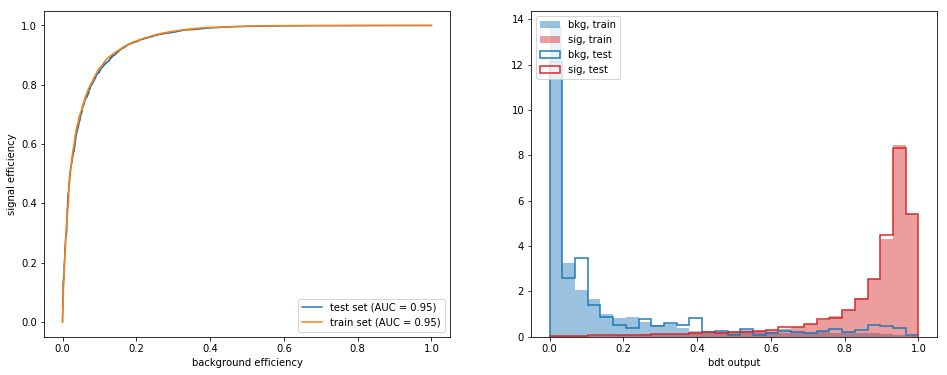
\includegraphics[width=.95\linewidth]{Dissertation/fig/bdt-performance.png}
\end{center}
\caption{Left: ROC curve showing BDT testing (blue) and training (orange) performance. Right: Background (blue) and signal (red) distributions versus BDT score for testing (outline) and training (filled).}
\label{fig:bdt-performance}
\end{figure}

\begin{figure}[htb]
\begin{center}
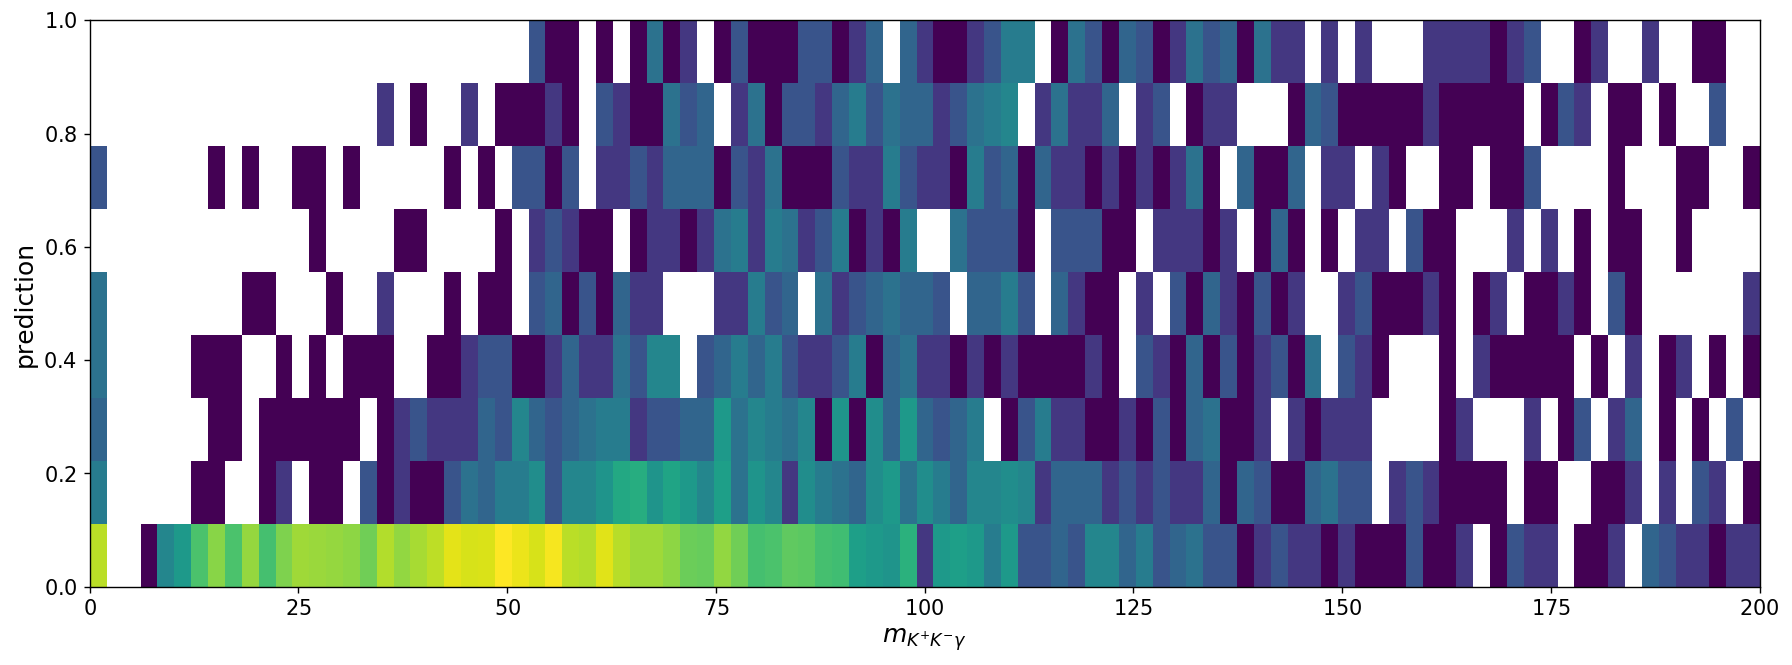
\includegraphics[width=.95\linewidth]{Dissertation/fig/bdt-bkgsculpt1.png}
\end{center}
\caption{Plot of the BDT score versus the reconstructed Higgs mass. A heavy correlation between high score and the true Higgs mass would suggest background is being sculpted.}
\label{fig:bdt-bkgsculpt1}
\end{figure}

\begin{figure}[htb]
\begin{center}
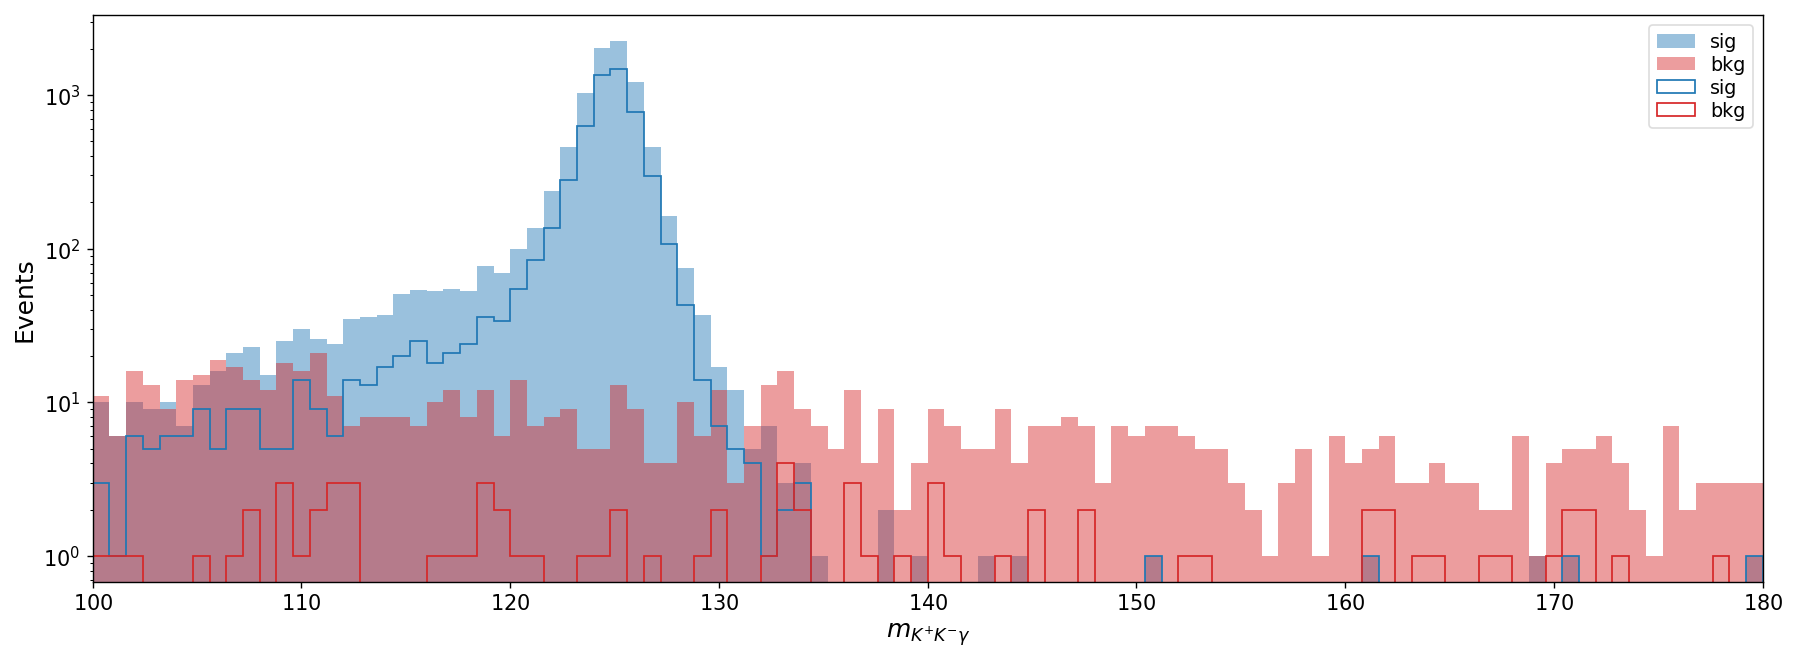
\includegraphics[width=.95\linewidth]{Dissertation/fig/bdt-bkgsculpt2.png}
\end{center}
\caption{Reconstructed Higgs mass distribution for signal (blue) and background (red) before (filled) and after (outline) requiring $D > 0.9$ where $D$ is the BDT discriminant.}
\label{fig:bdt-bkgsculpt2}
\end{figure}
\end{subsection}
\begin{subsection}{Comparison to Cut-Based Approach}
Based on the following basic study, we found that a Boosted Decision Tree (BDT) trained on Monte Carlo simulations of signal and background performed 20\% to 25\% better than traditional, cut-based methods. We determined an optimal BDT working point by sampling the BDT's ROC curve (generated using testing data and predictions) at each defined threshold value, then calculating an expected significance ($\sigma$) defined as:
\begin{equation}\label{expsig-eq}
    \sigma = \sqrt{2(s+b)\ln(1+s/b)-2s}
\end{equation}
\noindent where $s$ and $b$ are the number of signal and background events for a given threshold value. The optimal BDT working point is then given by the maximum $\sigma$-value. Next, we defined a general cut-based approach by the following cuts:
\begin{itemize}
    \item $1.0 < m_{\phi} < 1.04\textnormal{ GeV}$
    \item $\Delta R(K^{+}, K^{-}) < 0.015$
    \item $p_{T}(\phi) > 25\textnormal{ GeV}$
    \item $p_{T}(\gamma) > 40\textnormal{ GeV}$
    \item $I_{rel}(\phi) < 0.01$
\end{itemize}
\noindent Finally, we calculated the false-positive and true-positive rates of the cut-based methods and plotted them against the BDT's ROC curve. The results of this study are plotted in Fig. \ref{fig:bdt-vs-cuts}. Note that the terms BDT ``score," ``threshold," and ``discriminant" will be used interchangeably throughout the remainder of this paper with the understanding that they are the same quantity $D \in [0,1]$.

\begin{figure}[htb]
\begin{center}
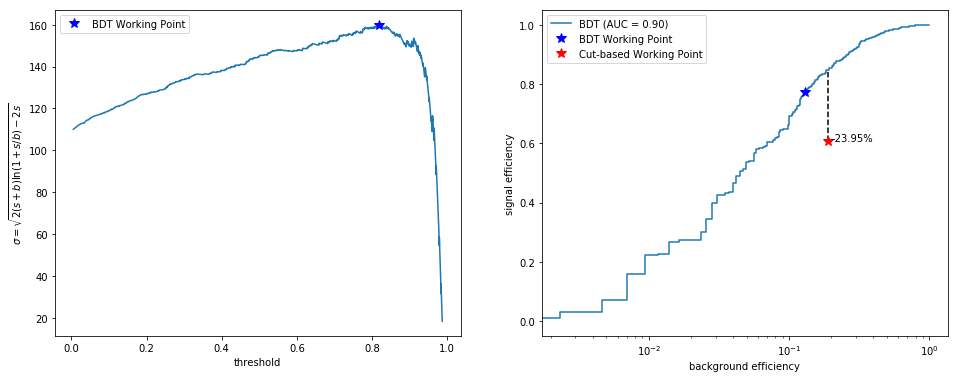
\includegraphics[width=.95\linewidth]{Dissertation/fig/bdt-vs-cuts.png}
\end{center}
\caption{Left: Expected significance ($\sigma$) versus BDT threshold value. Right: Comparison between an optimal BDT working point and cut-based method plotted on top of the BDT's ROC curve.}
\label{fig:bdt-vs-cuts}
\end{figure}
\end{subsection}
\begin{subsection}{Optimization for Data}
With the BDT validated, we proceeded to calculated a proper BDT working point for cutting on data. We noticed that the Monte Carlo samples were not properly modeling the data in the signal region of the BDT discriminant (Fig. \ref{fig:bdt-thresh-dist}). Thus, we concluded that we could not sample the BDT testing ROC curve for an effective working point. Instead, we fed the BDT ROC curve data as background in addition to signal Monte Carlo. We then sampled this distribution, calculated expected significance again using Eq. \ref{expsig-eq}, and took the best BDT working point to be at the threshold with maximum expected significance (Fig. \ref{fig:bdt-data-expsig}).

\begin{figure}[htb]
\begin{center}
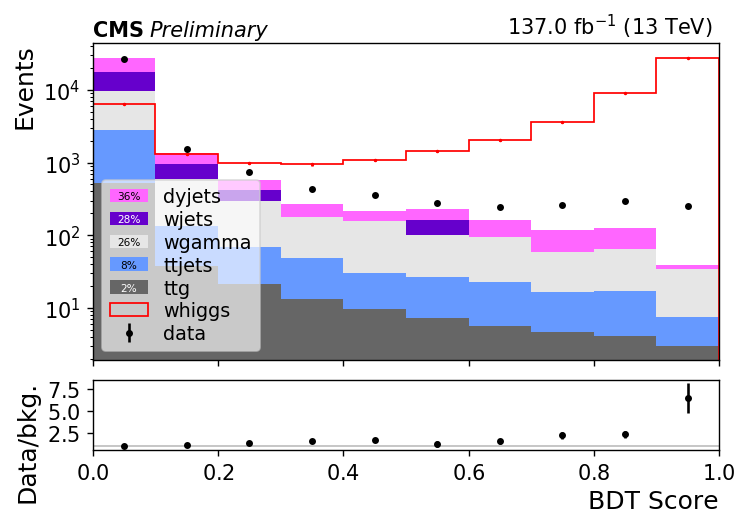
\includegraphics[width=.95\linewidth]{Dissertation/fig/bdt-threshBySample.png}
\end{center}
\caption{Stacked BDT discriminant distribution plot by sample.}
\label{fig:bdt-thresh-dist}
\end{figure}

\begin{figure}[htb]
\begin{center}
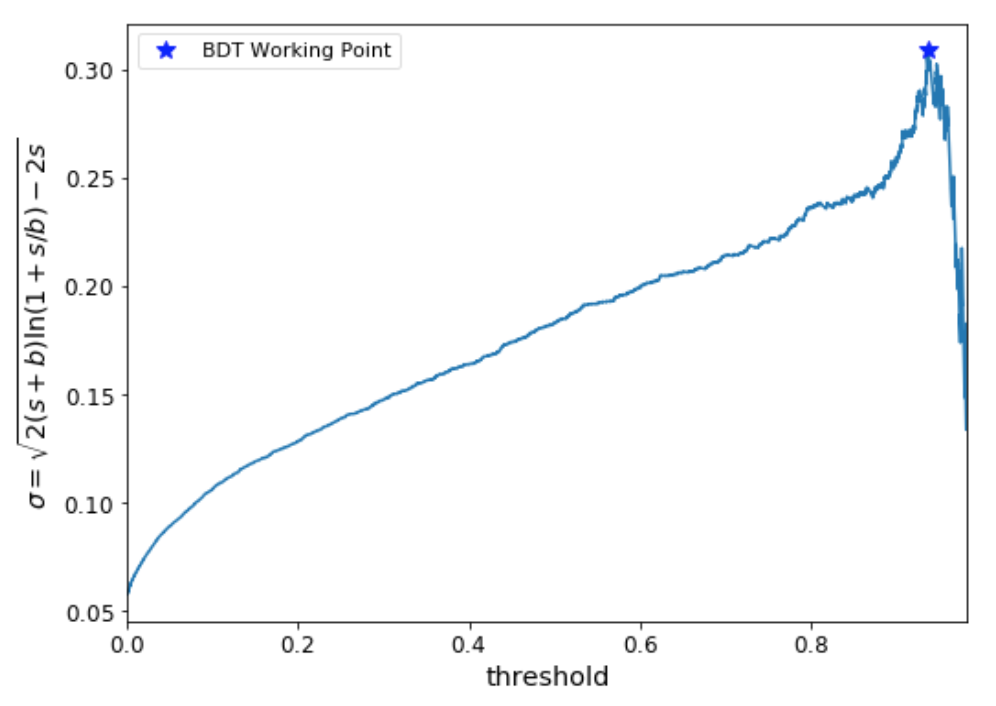
\includegraphics[width=.95\linewidth]{Dissertation/fig/bdt-data-expsig.png}
\end{center}
\caption{Expected significance versus BDT threshold.}
\label{fig:bdt-data-expsig}
\end{figure}

\end{subsection}
\end{section}

\begin{section}{Results}
Lorem ipsum dolor sit amet, consectetur adipiscing elit. Quisque eu eros nisl. Donec sollicitudin nisl nisi, sit amet rutrum nibh faucibus sit amet. In a efficitur dui. Nunc at sagittis urna. Quisque venenatis nec risus quis eleifend. Fusce id nulla in urna tristique iaculis. In et consectetur risus, nec commodo justo. In augue enim, efficitur ac commodo quis, tempus ac arcu. Sed porta dolor ultrices, pellentesque tellus eu, mollis mi. Phasellus et condimentum odio. Curabitur condimentum rhoncus sem, eget sagittis eros rhoncus sit amet. Class aptent taciti sociosqu ad litora torquent per conubia nostra, per inceptos himenaeos. Maecenas ac felis aliquam orci eleifend faucibus vitae sit amet mauris. Fusce vel magna mi. Aenean commodo pellentesque tellus, ut iaculis est auctor et.
Aliquam porttitor justo dolor. Duis ut ex lacinia, vulputate dui a, molestie lorem. Vestibulum elementum lectus vel mollis iaculis. Cras ante purus, pellentesque sit amet sem sed, convallis dapibus est. Aenean vehicula mollis bibendum. Integer aliquet condimentum luctus. Suspendisse vitae rhoncus justo.
\end{section}

\begin{figure}[htb]
\begin{center}
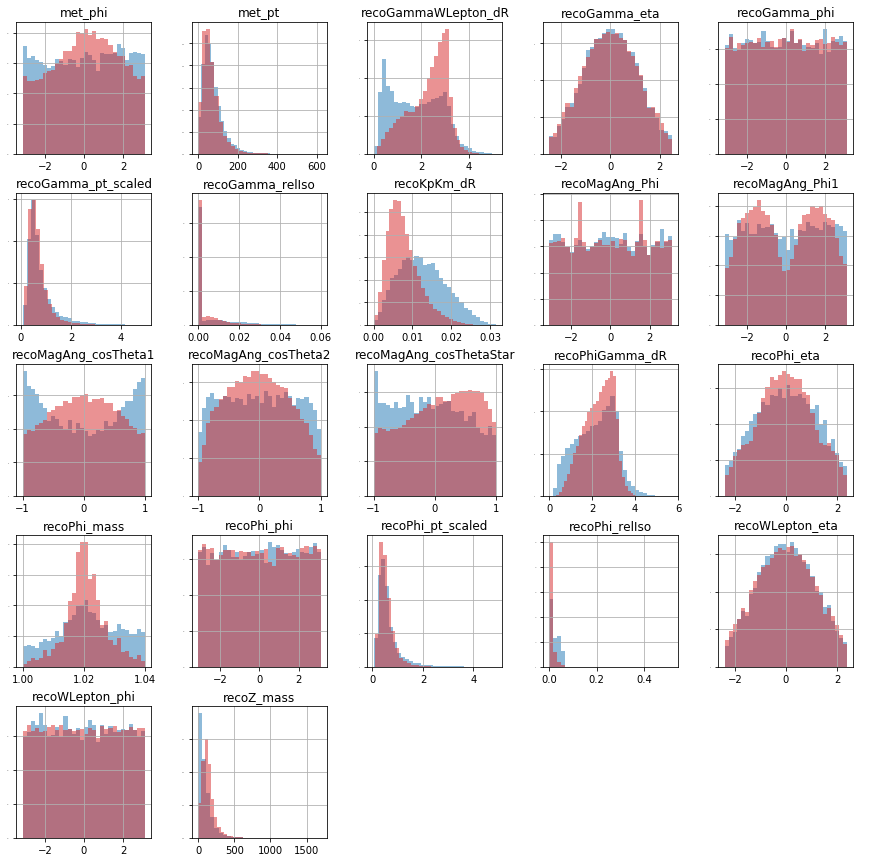
\includegraphics[width=.95\linewidth]{Dissertation/fig/bdt-training.png}
\end{center}
\caption{Preliminary histograms for every feature used to train the BDT. These were drawn before any weights are applied, so they do not completely represent what the BDT saw, however they do provide some insight into the motivation behind the BDT's variable rankings.}
\label{fig:bdt-training}
\end{figure}